\let\negmedspace\undefined
\let\negthickspace\undefined
\documentclass[journal]{IEEEtran}
\usepackage[a5paper, margin=10mm, onecolumn]{geometry}
%\usepackage{lmodern} % Ensure lmodern is loaded for pdflatex
\usepackage{tfrupee} % Include tfrupee package

\setlength{\headheight}{1cm} % Set the height of the header box
\setlength{\headsep}{0mm}     % Set the distance between the header box and the top of the text

\usepackage{gvv-book}
\usepackage{gvv}
\usepackage{cite}
\usepackage{amsmath,amssymb,amsfonts,amsthm}
\usepackage{algorithmic}
\usepackage{graphicx}
\usepackage{textcomp}
\usepackage{xcolor}
\usepackage{txfonts}
\usepackage{listings}
\usepackage{enumitem}
\usepackage{mathtools}
\usepackage{gensymb}
\usepackage{comment}
\usepackage[breaklinks=true]{hyperref}
\usepackage{tkz-euclide} 
\usepackage{listings}
% \usepackage{gvv}                                        
\def\inputGnumericTable{}                                 
\usepackage[latin1]{inputenc}                                
\usepackage{color}                                            
\usepackage{array}                                            
\usepackage{longtable}                                       
\usepackage{calc}                                             
\usepackage{multirow}                                         
\usepackage{hhline}                                           
\usepackage{ifthen}                                           
\usepackage{lscape}
\begin{document}

\bibliographystyle{IEEEtran}
\vspace{3cm}

\title{1-1.10-31}
\author{EE24BTECH11062 - Homa Harshitha Vuddanti
}
% \maketitle
% \newpage
% \bigskip
{\let\newpage\relax\maketitle}

\renewcommand{\thefigure}{\theenumi}
\renewcommand{\thetable}{\theenumi}
\setlength{\intextsep}{10pt} % Space between text and floats


\numberwithin{equation}{enumi}
\numberwithin{figure}{enumi}
\renewcommand{\thetable}{\theenumi}


\textbf{Question}:\\
Find the direction cosines of the line passing through the two points $\myvec{-2\\4\\-5}$ and $\myvec{1\\2\\3}$.
\\
\textbf{Solution: }\\
Given two points,
\begin{table}[h!]    
  \centering
  \begin{tabular}[12pt]{ |c| c|}
    \hline
    \textbf{Variable} & \textbf{Description}\\ 
    \hline
    $a$ & $x$-coordinate of point B\\
    \hline 
    $b$ & $y$-coordinate of point C\\
    \hline
    \end{tabular}


  \caption{Variables used}
  \label{1-1.10-31-table}
\end{table}
The direction vector is given as,
\begin{align}
    m&=\vec{B}-\vec{A}\label{1-1.10-31-1}\\
    m&=\myvec{1\\2\\3}-\myvec{-2\\4\\-5}\\
    m&=\myvec{3\\-2\\8}\label{1-1.10-31-2}
\end{align}
Direction cosines are given by a unit vector in that direction-
\begin{align}
    \frac{AB}{\norm{AB}}&=\frac{m}{\norm{m}}\label{1-1.10-31-3}
\end{align}
 \begin{align}
    \norm{m}&=\sqrt{m^\top m}\\
    \norm{m}&=\myvec{3\\-2\\8}^\top \myvec{3\\-2\\8}\\
   \norm{m}&=\sqrt{77}\label{1-1.10-31-4}
\end{align}
 From equations \eqref{1-1.10-31-3} and \eqref{1-1.10-31-4}, 
 direction cosines are-
\begin{align}
\frac{1}{\sqrt{77}}\myvec{3\\-2\\8}=\myvec{\frac{3}{\sqrt{77}}\\\frac{-2}{\sqrt{77}}\\\frac{8}{\sqrt{77}}}
\end{align}
\begin{figure}[h!]
   \centering
   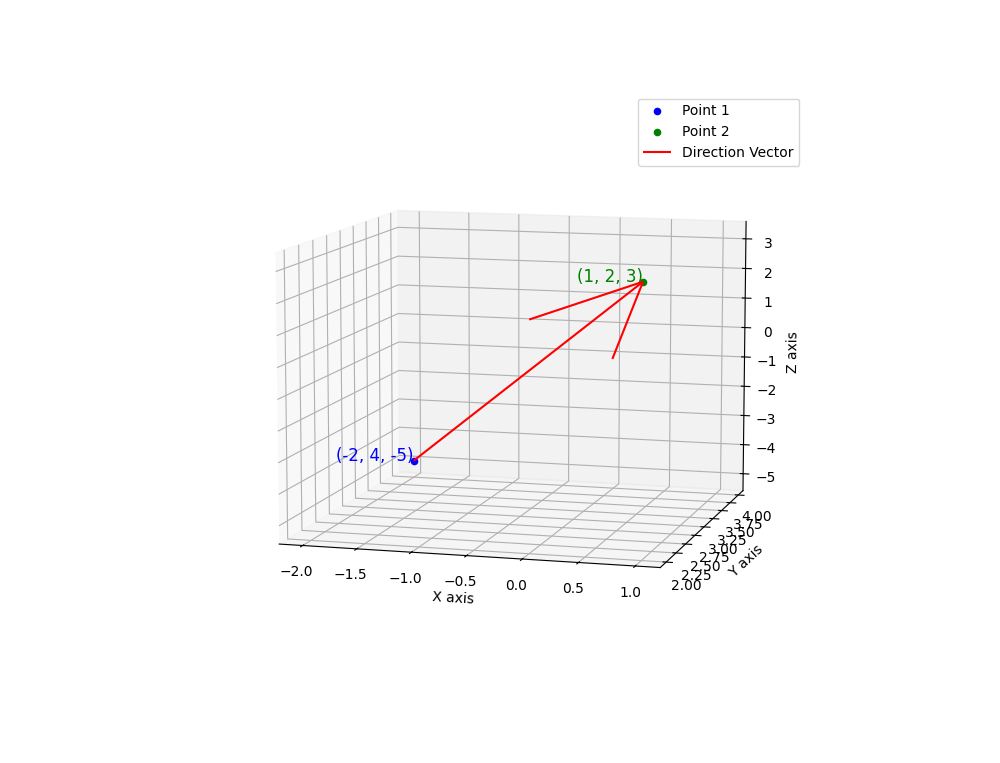
\includegraphics[width=1.1\columnwidth]{Figs/Figure_1.png}
   \caption{Plot}
   \label{1-1.10-31-fig-1}
\end{figure}
\end{document}  





